\newpage

\section{ワイヤ駆動式柔軟外皮装着型魚ロボット}
本章では先行研究\cite{kyu}や試作ロボットから得られた知見をもとに本研究で開発した,柔軟外皮がリンクの動きに追従し,完全防水可能かつメンテンナンス性を向上させた,柔軟外皮装着型
のワイヤ駆動式魚ロボットについて述べる.
\subsection{ロボット概要}
図\ref{fig:fishrobo_with}に開発した機体の外観を,図\ref{fig:kouzou}に構造を示す.開発した魚ロボットは体長470 mm,重量は重り(25 g)を含めて710 gである.
\begin{figure}[htbp]
    \centering  
    \begin{subfigure}[b]{0.85\linewidth}
        \centering
        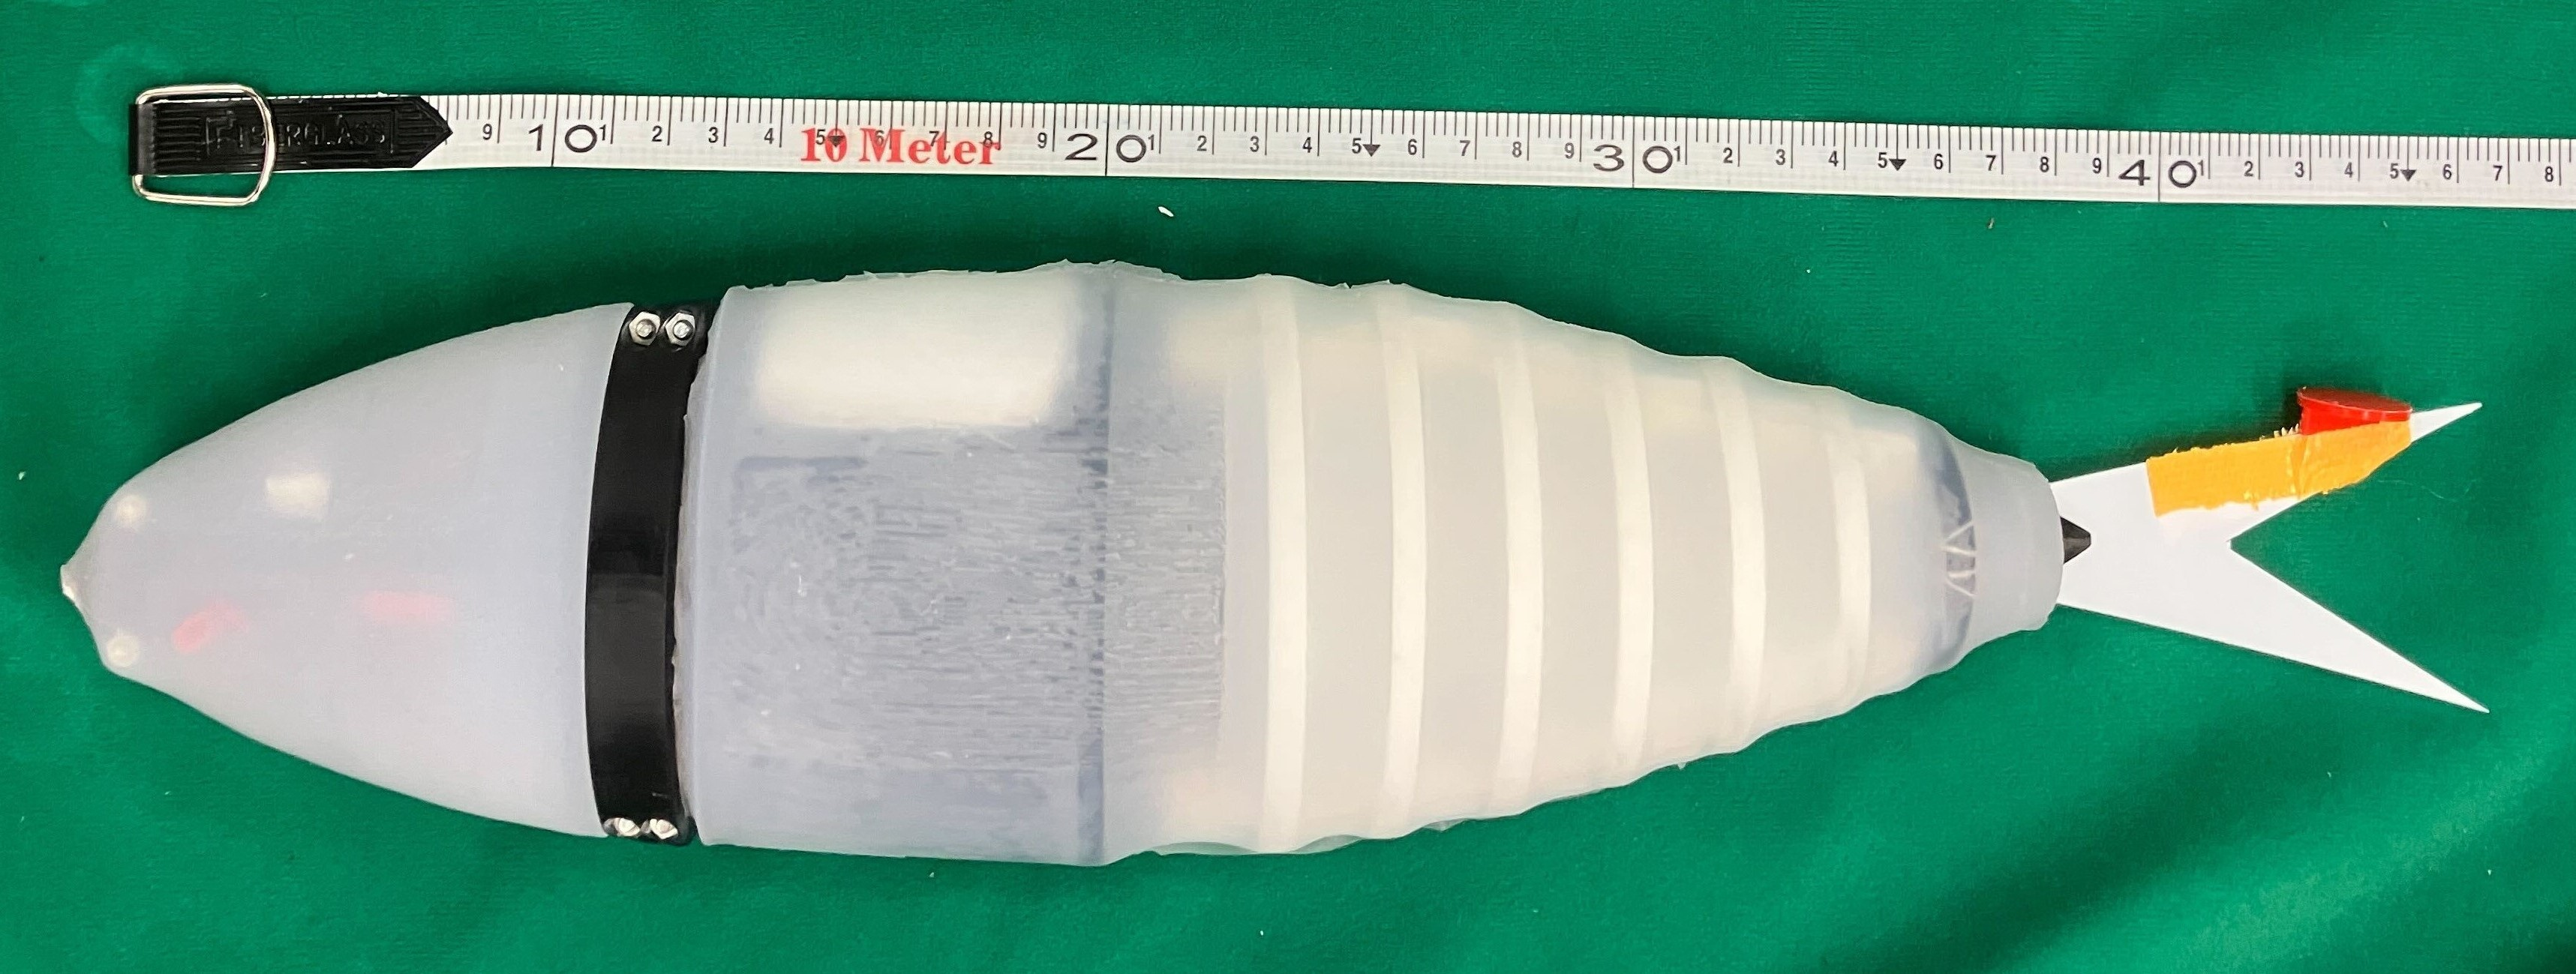
\includegraphics[width=0.9\linewidth]{chapters/picture/withskin.jpg}
        \subcaption{外皮装着時}
        \label{fig:fishrobo_with}
    \end{subfigure}
    \begin{subfigure}[b]{0.85\linewidth}
        \centering
        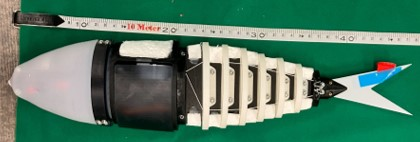
\includegraphics[width=0.9\linewidth]{chapters/picture/without_skin.jpg}
        \subcaption{胴体部の柔軟外皮未装着時}
        \label{fig:fishrobo_less}
    \end{subfigure}
    \begin{subfigure}[b]{0.85\linewidth}
        \centering
        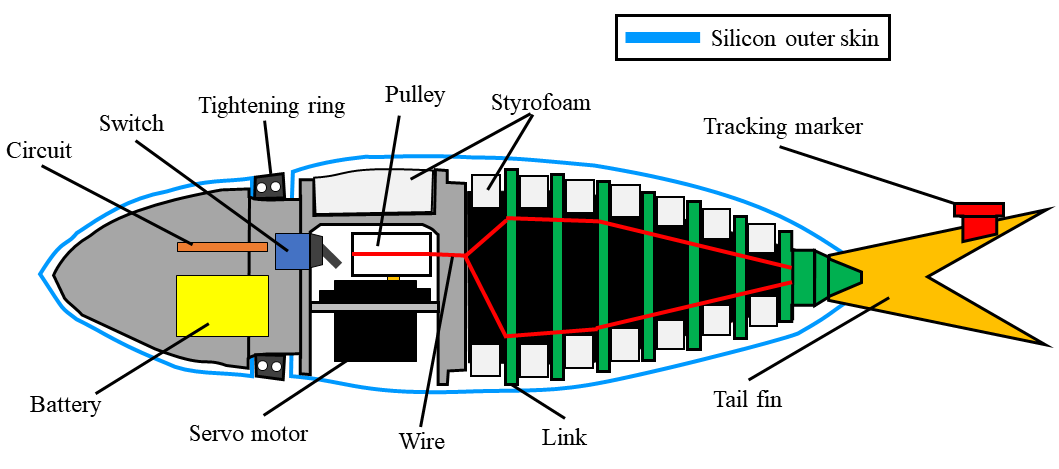
\includegraphics[width=0.9\linewidth]{chapters/picture/fish.png}
        \caption{開発したロボットの構造}
        \label{fig:kouzou}
    \end{subfigure}
    \caption{開発したロボット}
    \label{fig:gaikan}
\end{figure}
ロボットの外形は
昨年度卒業研究においてアジのスキャンデータ(図\ref{fig:data_scan})から作製したモデルデータ(図\ref{fig:data_model})をもとに作製し,サイズは2倍とした.本機体は頭部・胴体
部・外皮の3つからなり,頭部と胴体部をそれぞれ別の柔軟外皮で包む構造になっている.また,頭部は防水区画とし,胴体部は水中姿勢を水平にするために浸水させた.

\begin{figure}[t]
    \centering
    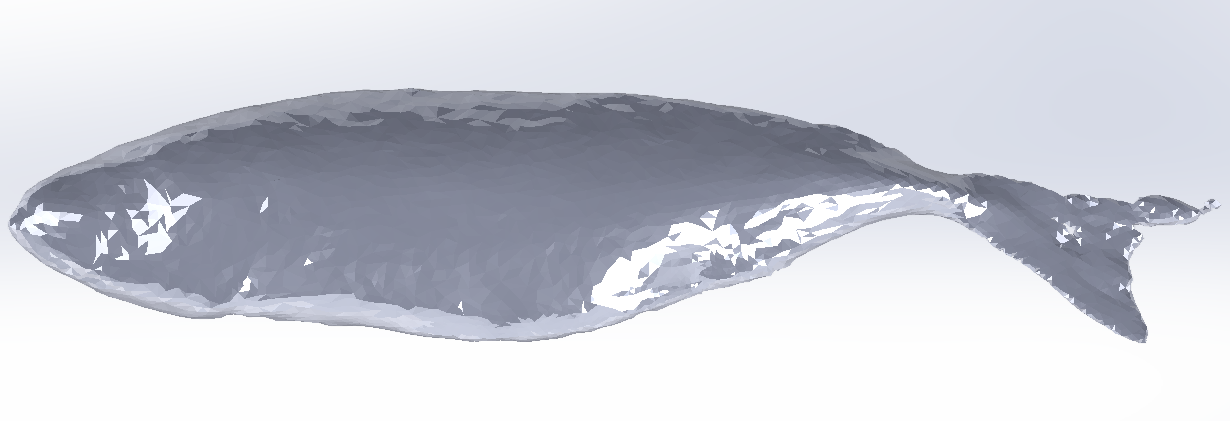
\includegraphics[width=0.7\linewidth]{chapters/picture/scan.png}
    \caption{アジのスキャンデータ}
    \label{fig:data_scan}
\end{figure}
\begin{figure}[t]
    \centering
    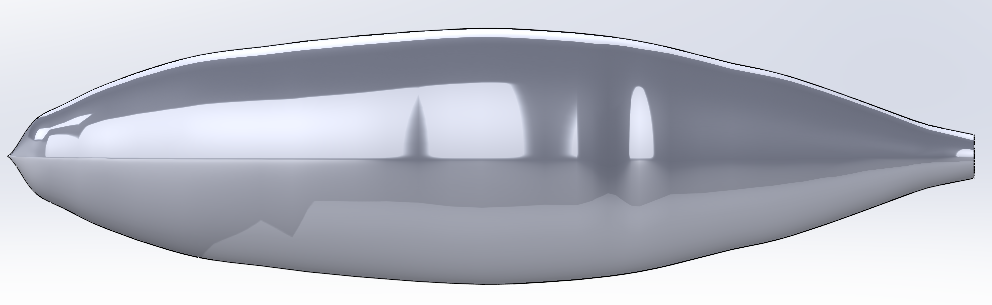
\includegraphics[width=0.7\linewidth]{chapters/picture/fishkinji2.png}
    \caption{アジのモデルデータ}
    \label{fig:data_model}
\end{figure}

\subsection{頭部}
頭部はフレーム部分とシリコン製の外皮部分からなる.フレーム部分は光造形方式の3Dプリンタで作製しており,胴体前部と一体となっている.フレーム内部にはバッテリーと制御回路を搭載しており,使用するバッテリー,マイコン共に試作機と同じものを用いた.バッテリーと
マイコンを搭載する都合上頭部を防水する必要があり,試作機から得た知見をもとに今回はOリングによる防水ではなく,シリコン製の外皮を用いて防水を行った.
防水方法としてはシリコン製の外皮を頭部にかぶせ,根元を防水リングによって締め付けることで防水を行った(図\ref{fig:bousui}).防水リングのサイズは\cite{juuiti}を参考に締め付ける部分が
短径,長径ともに10%つぶせるように設計した.
また,試作機と同様に防水実験を1回行ったが,内部に貼ったシールはどれも赤く染まらず,完全な防水ができた(図\ref{fig:bousui_test}).
また,フレーム部分は上部と下部のカバーが開くようになっており,メンテナンス性向上のためにねじ止めではなくワンタッチでカバーを開閉できるようにしている
(図\ref{fig:head_open},\ref{fig:rock}).
それに加えて制御回路とバッテリーを取り出しやすくするためにねじで固定するのではなく,図\ref{fig:toubu_kiban},図\ref{fig:toubu_battery}のように溝にはめストッパーをつける
ことで頭部に配置している.

\begin{figure}[t]
    \centering
    \begin{tabular}{cc}
        \begin{minipage}[b]{0.33\linewidth}
            \centering
            \setPicture{bousui.pdf}
            \subcaption{防水構造}
            \label{fig:bousui_kouzou} 
        \end{minipage}
        \begin{minipage}[b]{0.33\linewidth}
            \centering
            \setPicture{jissai.jpg}
            \subcaption{実際の様子}
            \label{fig:bousui_jissai} 
        \end{minipage}
    \end{tabular}
    \caption{頭部防水について}
    \label{fig:bousui}
\end{figure}
\begin{figure}[t]
    \centering
    \begin{tabular}{ccc}
        \begin{minipage}[b]{0.25\linewidth}
            \centering
            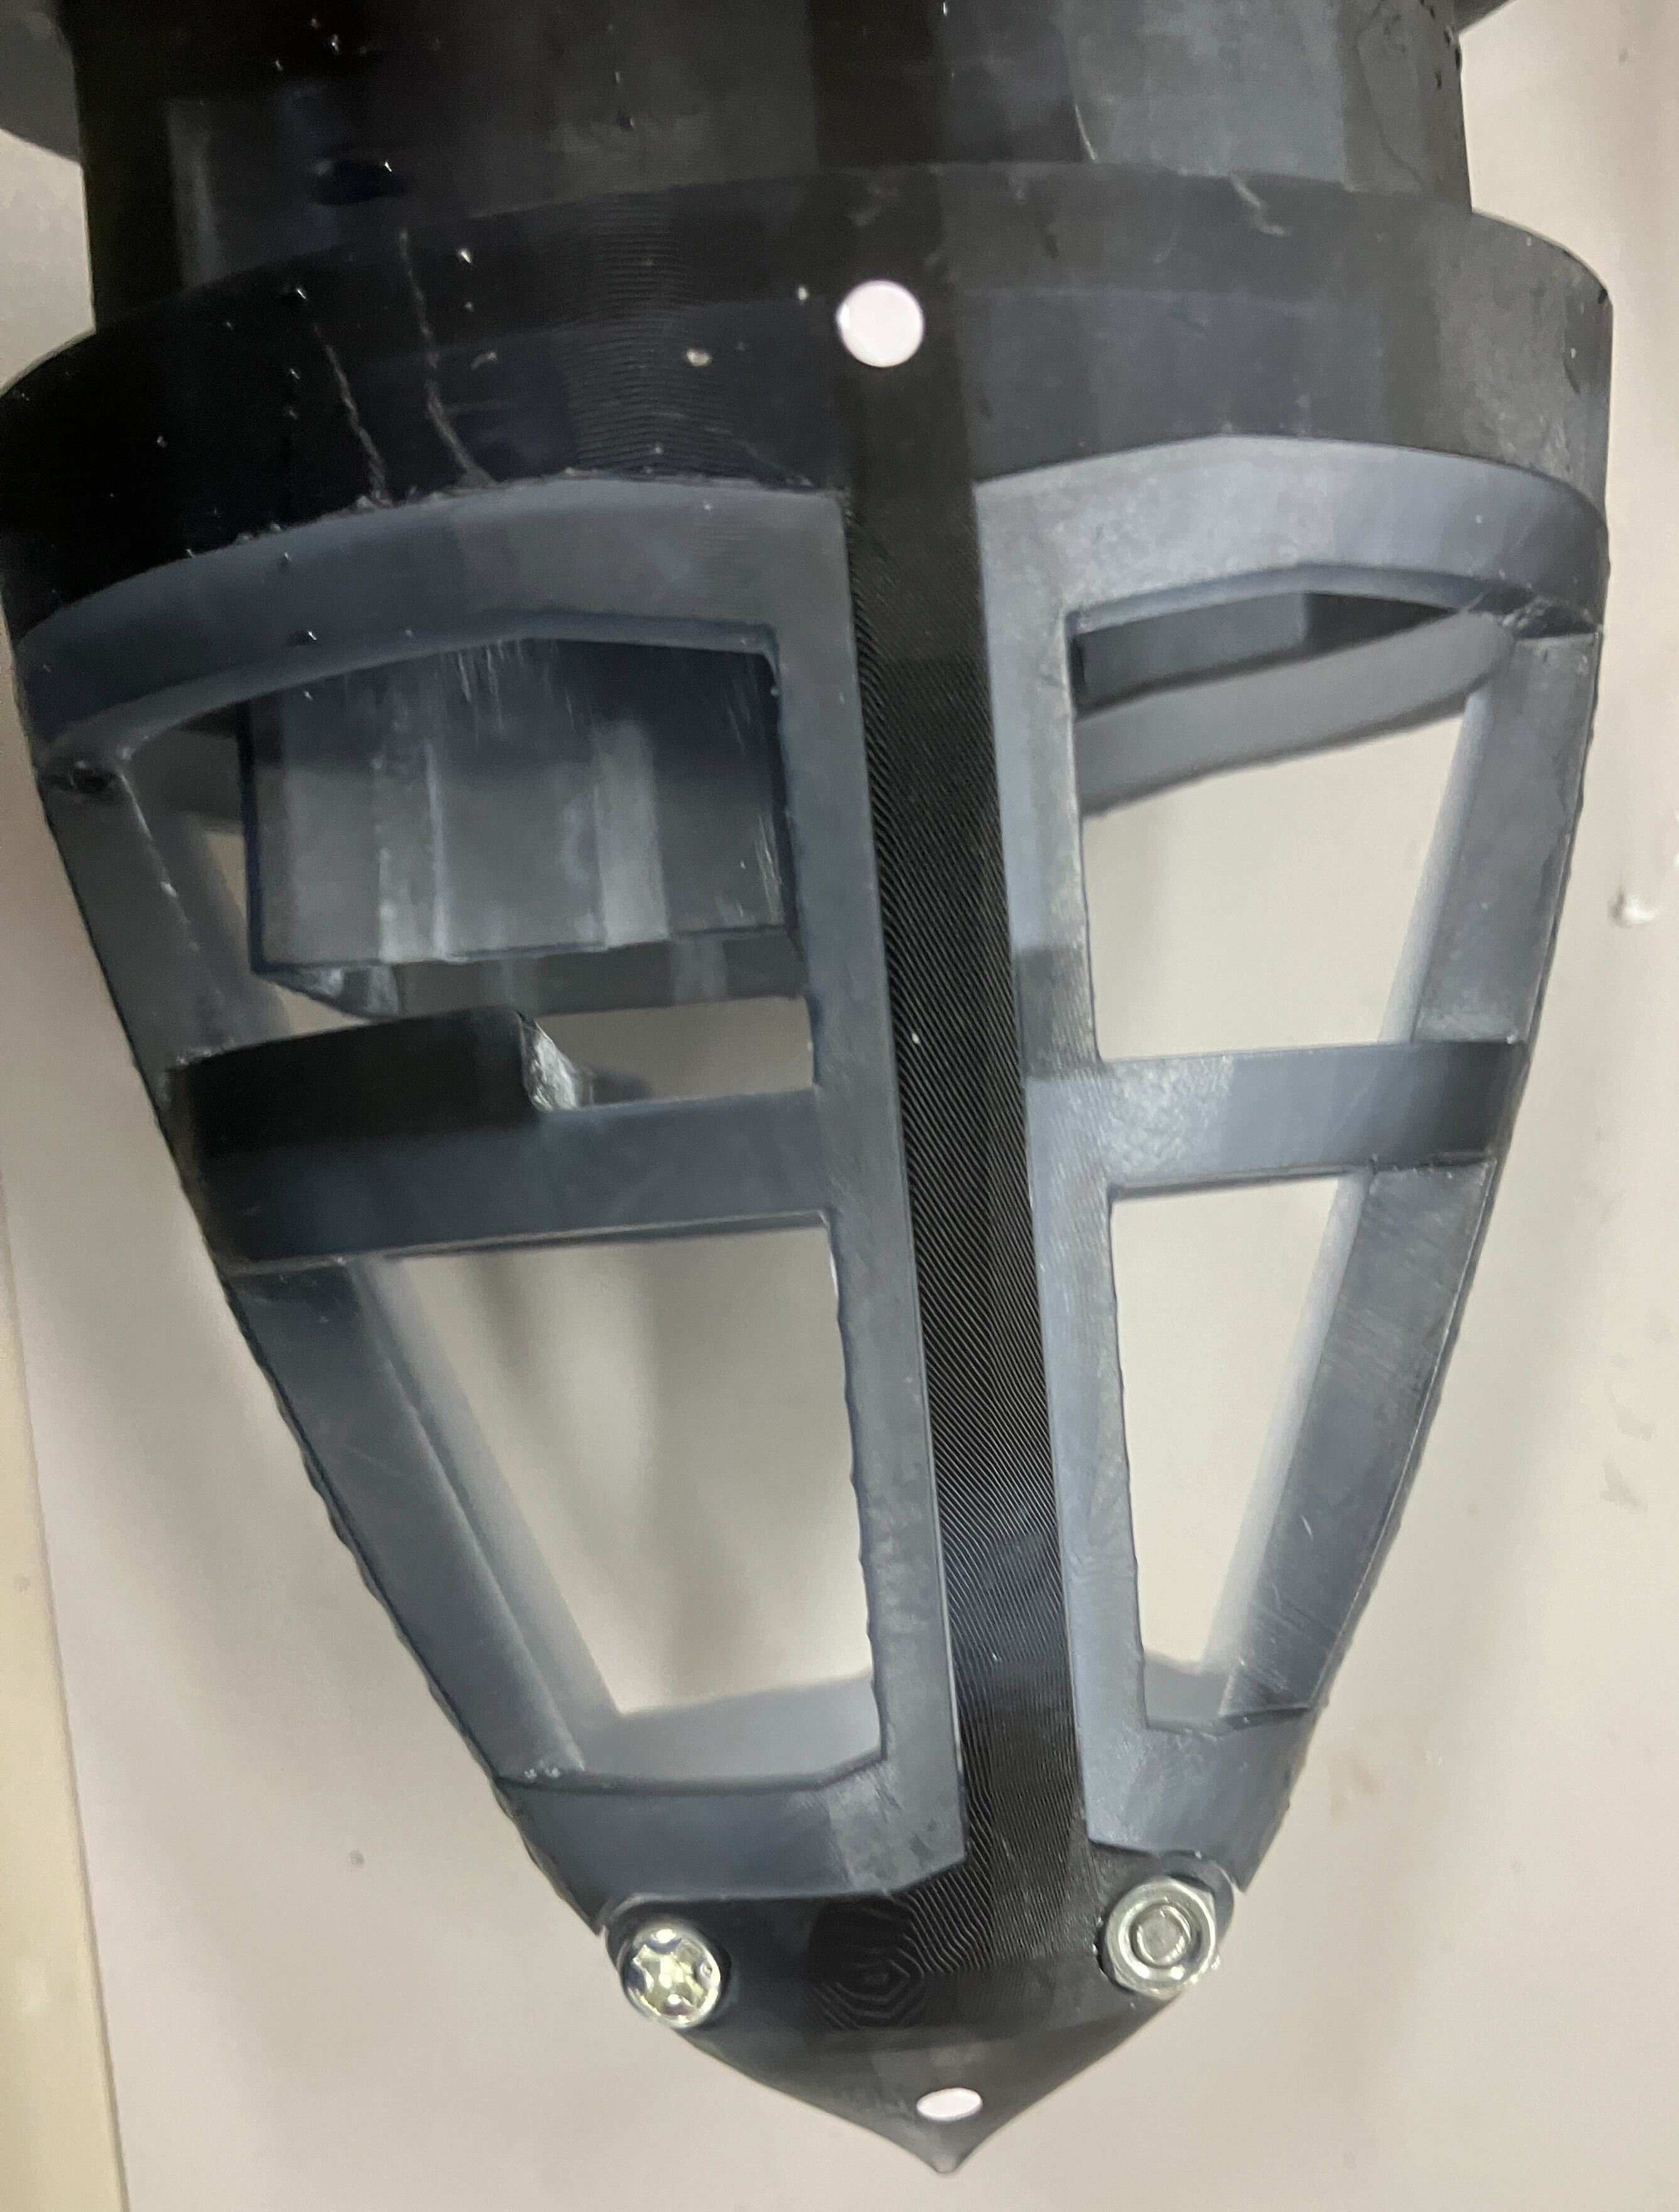
\includegraphics[width=0.7\linewidth]{chapters/picture/bousui_soku.jpg}
            \subcaption{頭部側面}
            \label{fig:toubu_soku}
        \end{minipage}
        \begin{minipage}[b]{0.25\linewidth}
            \centering
            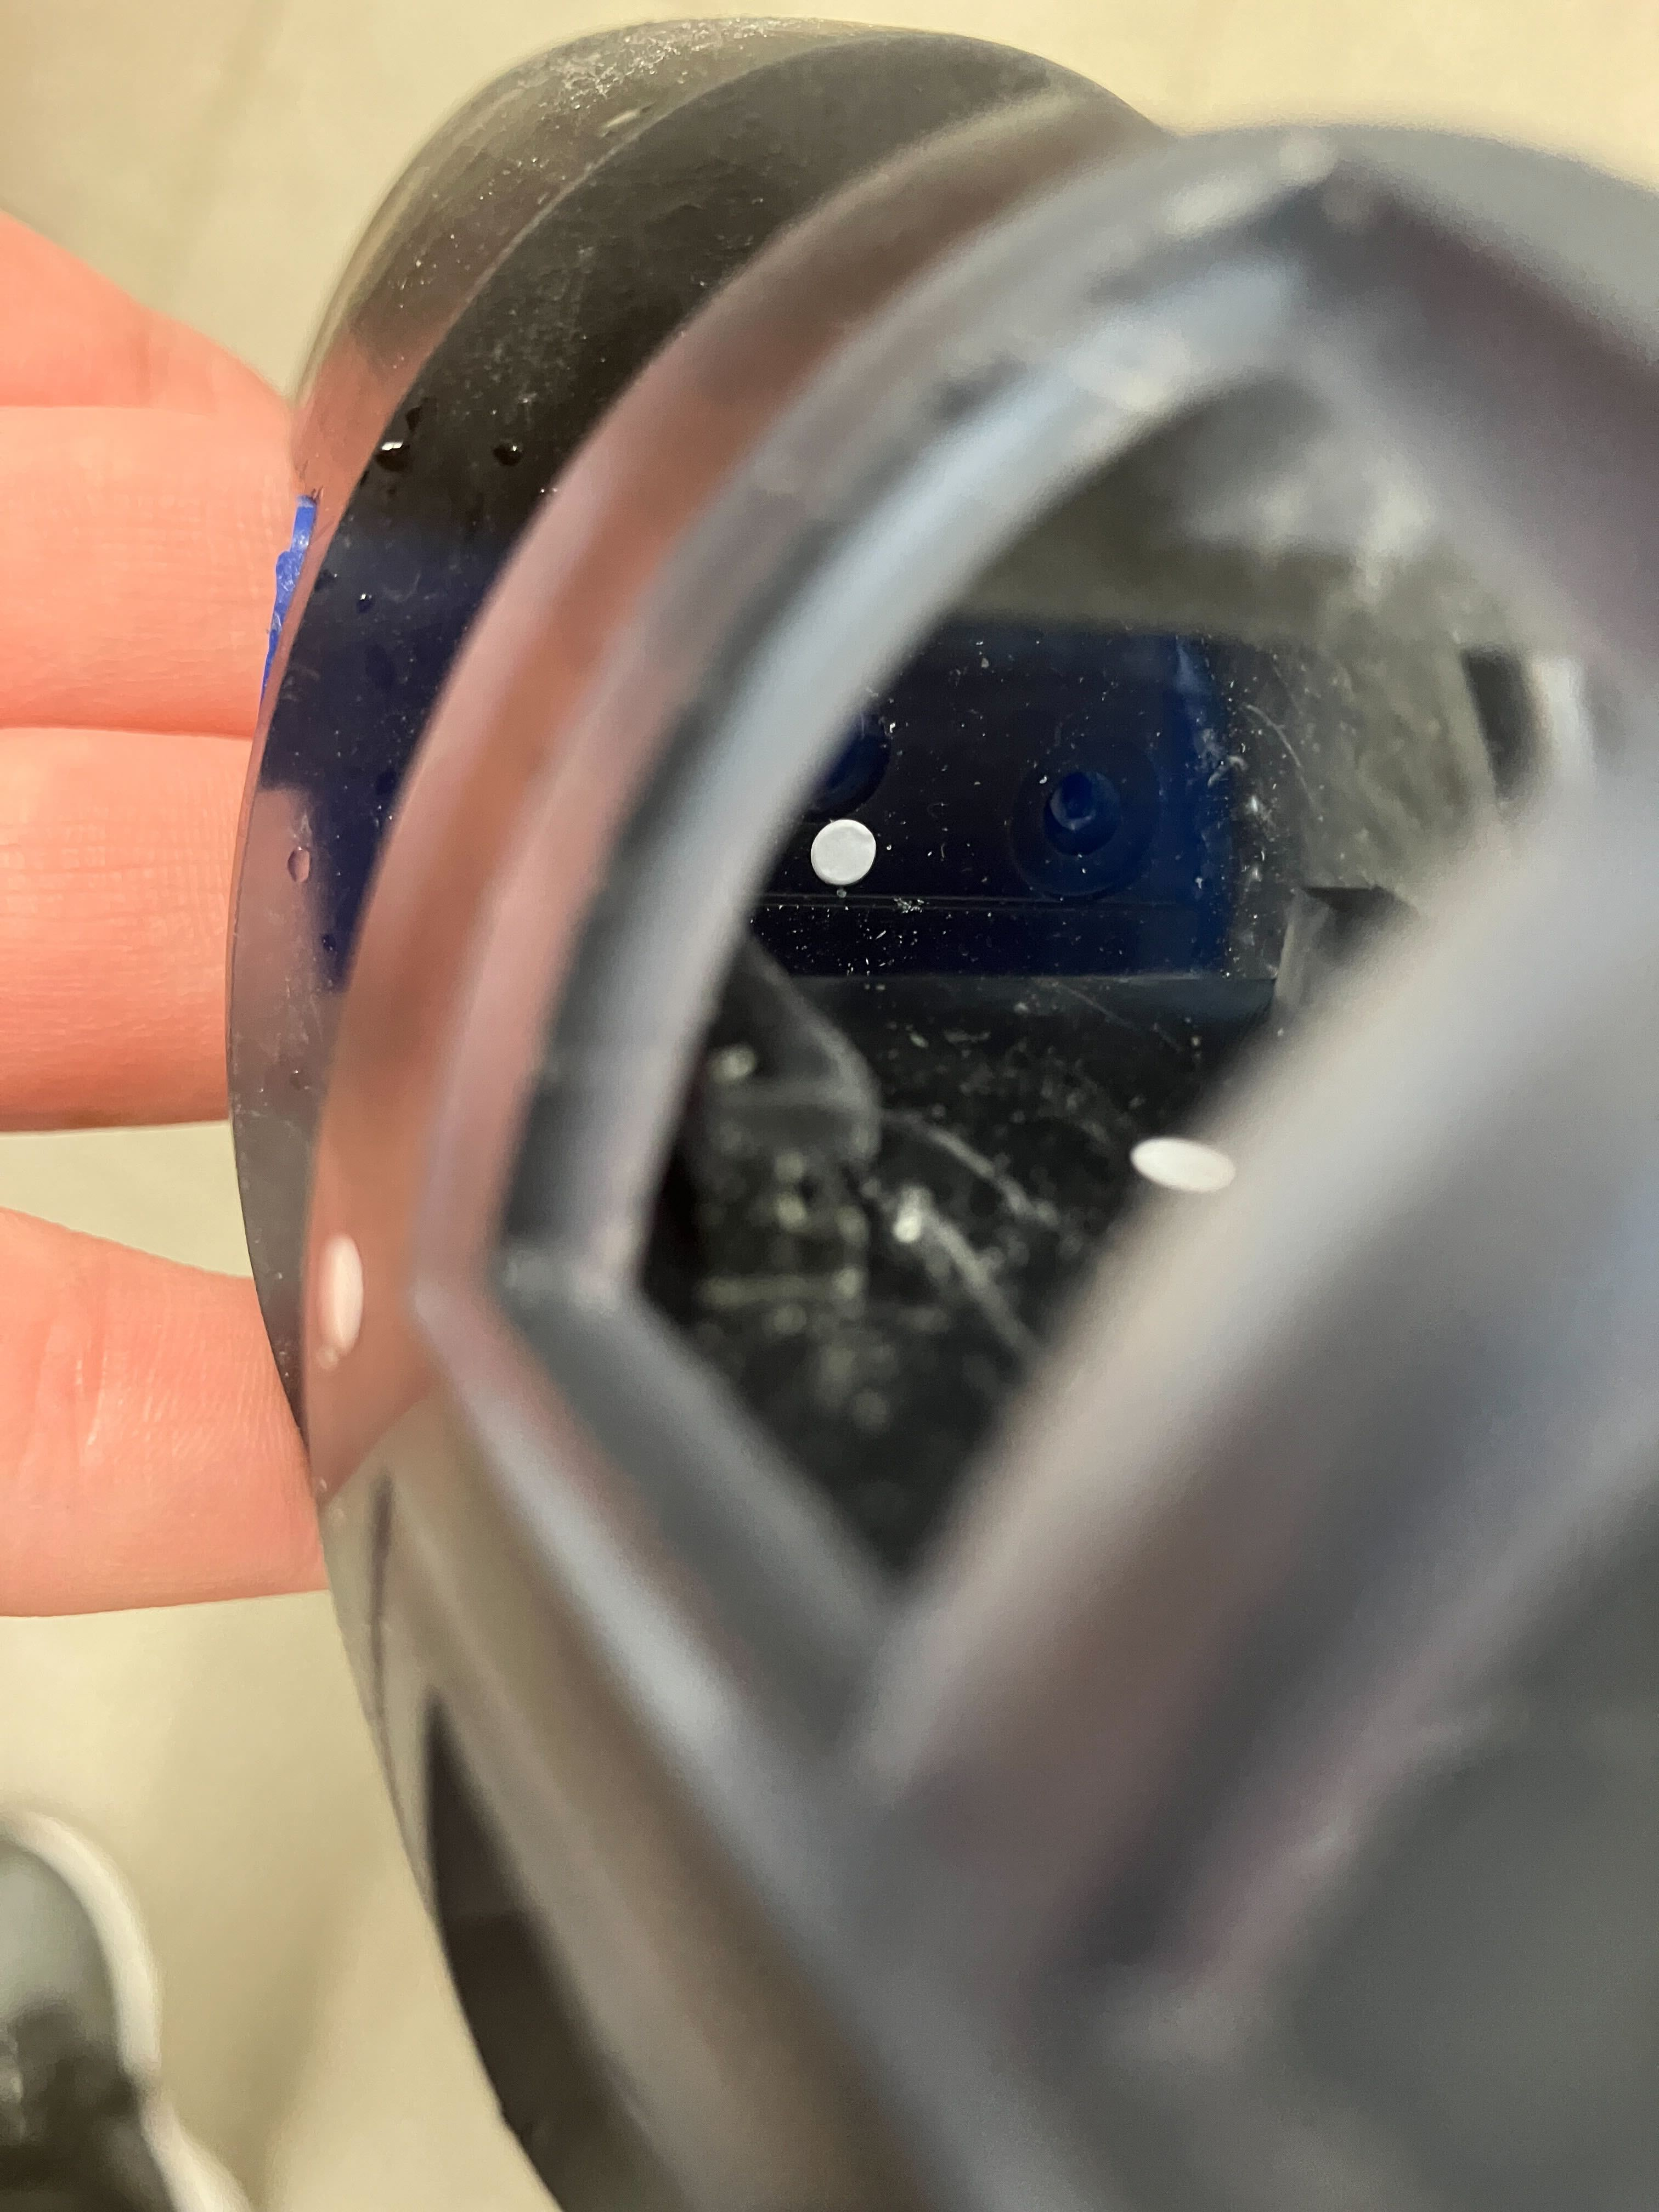
\includegraphics[width=0.7\linewidth]{chapters/picture/bousui_naka.jpg}
            \subcaption{頭部内側}
            \label{fig:toubu_uti}
        \end{minipage}
        \begin{minipage}[b]{0.25\linewidth}
            \centering
            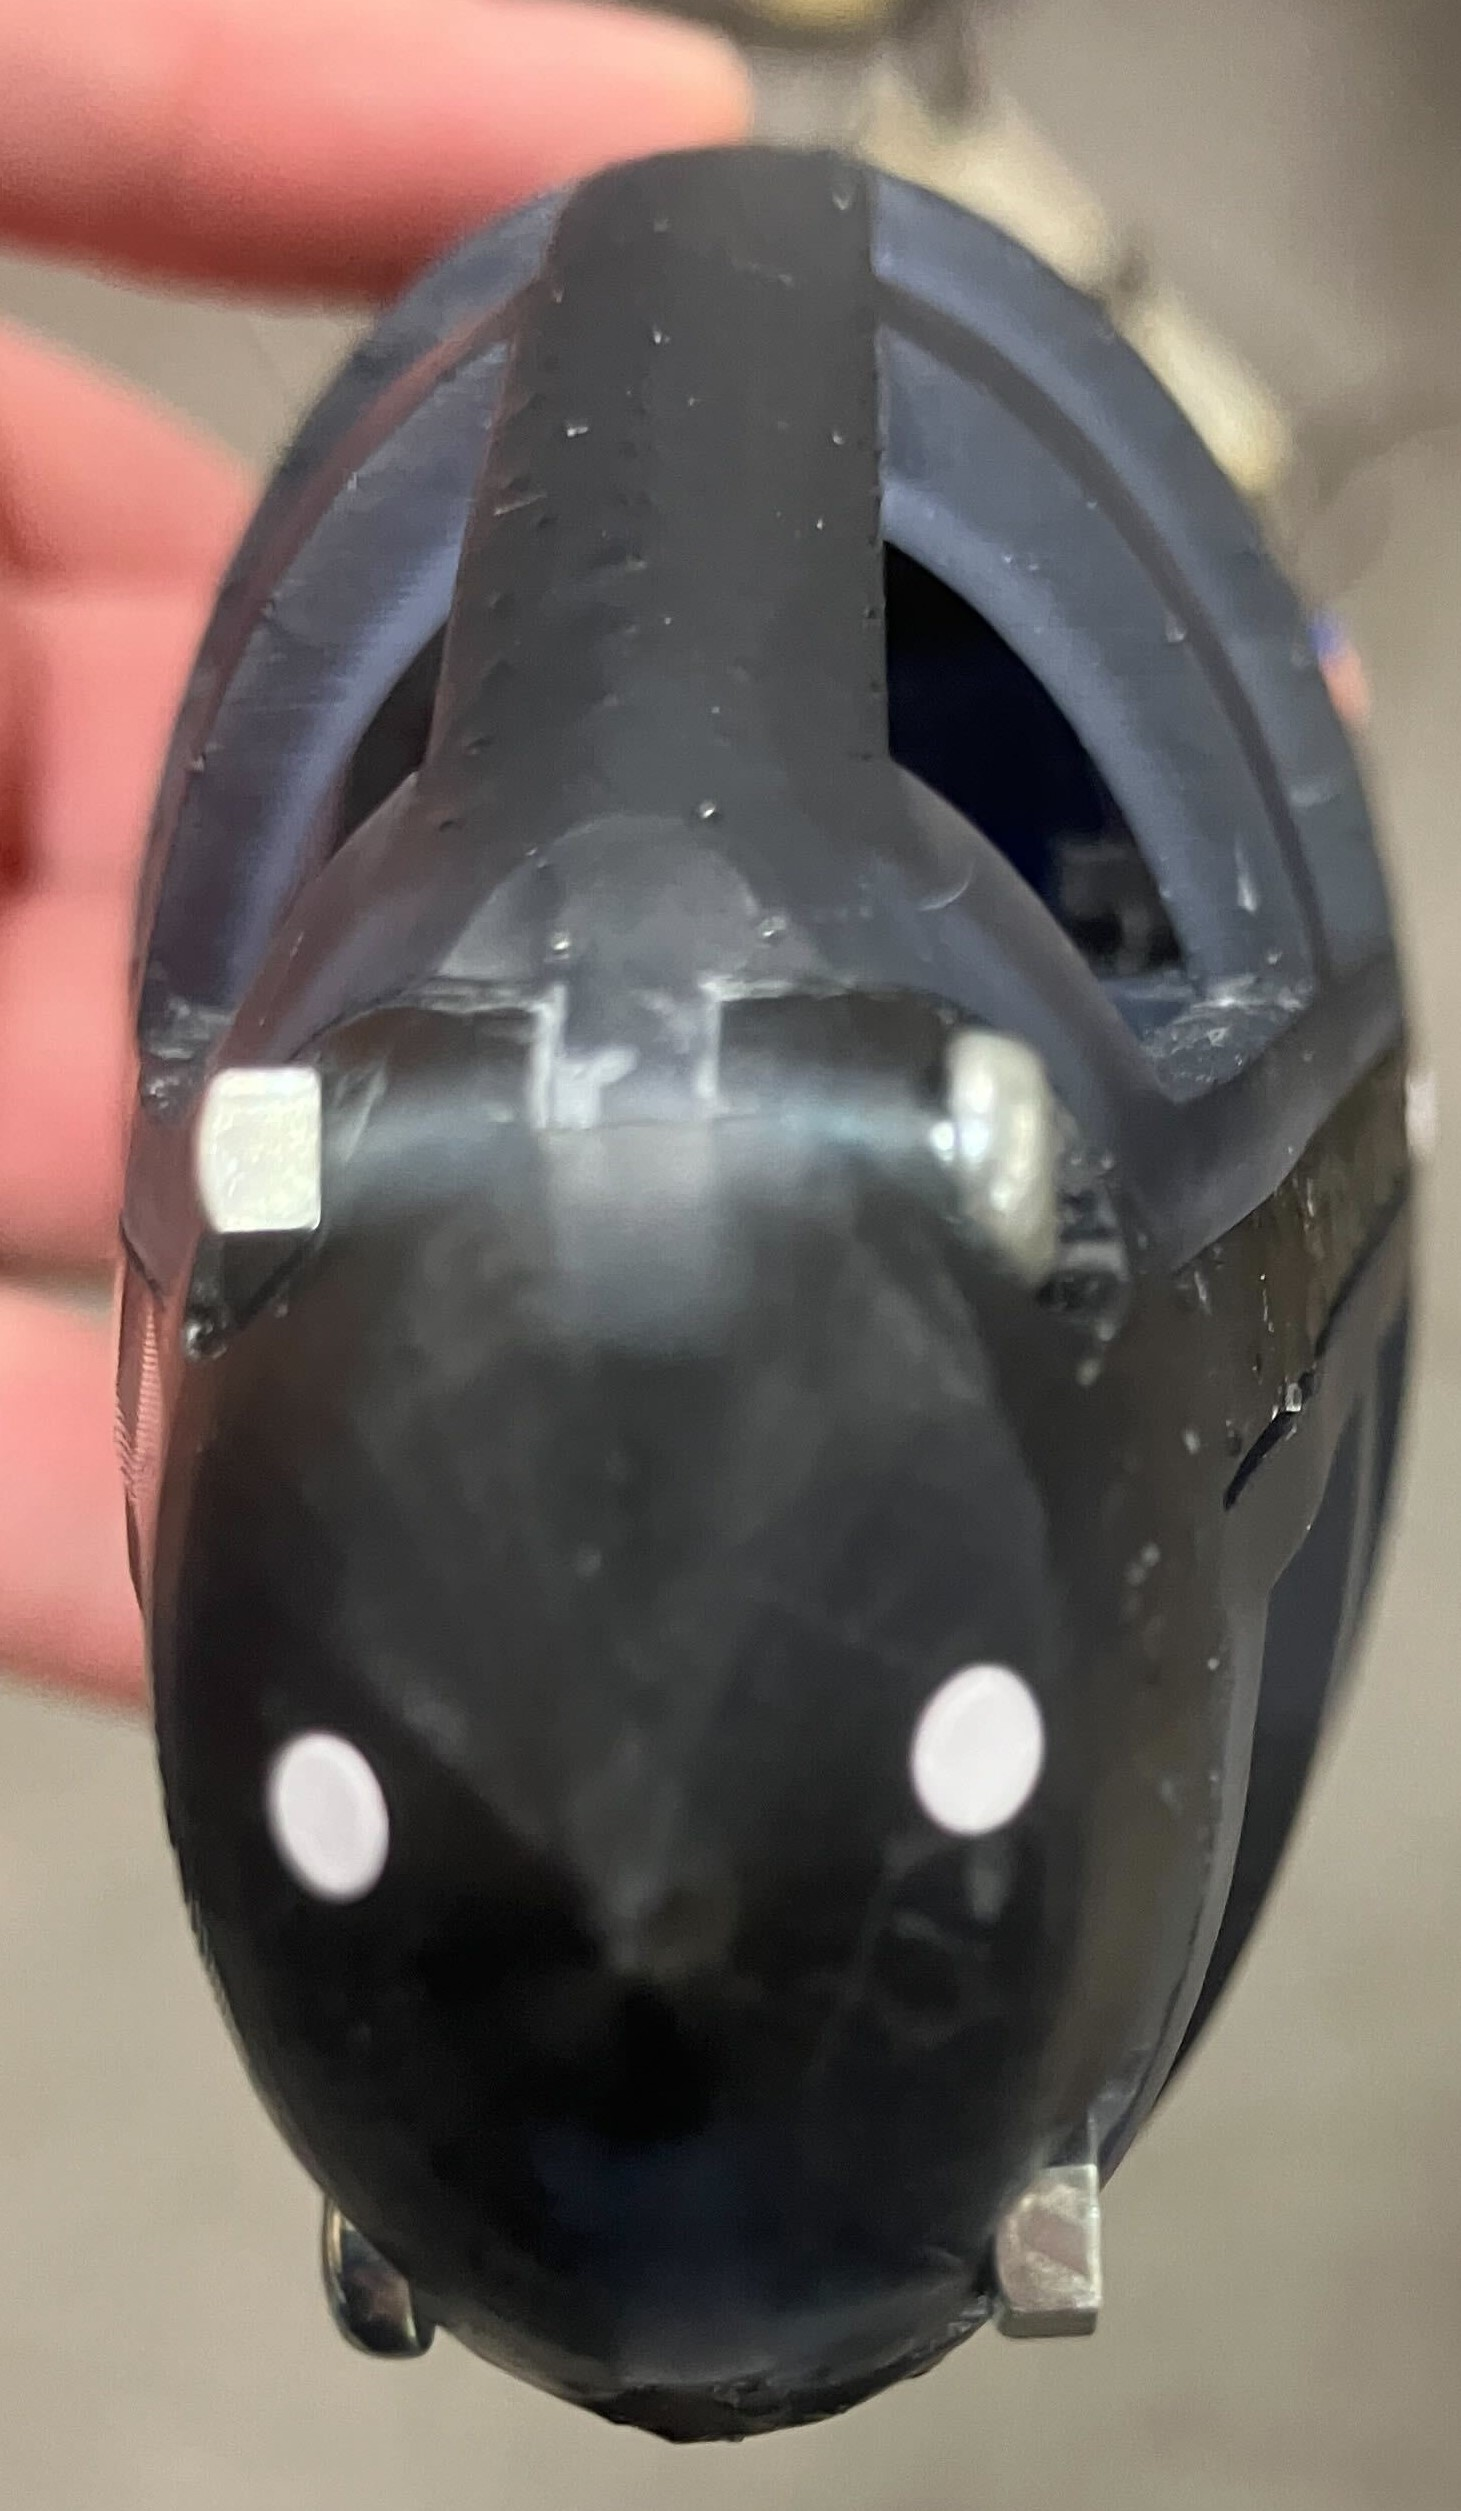
\includegraphics[width=0.6\linewidth]{chapters/picture/bousui_sentou.jpg}
            \subcaption{頭部先端}
            \label{fig:toubu_sentan}
        \end{minipage}
    \end{tabular}
    \caption{防水実験後のシールの様子}
    \label{fig:bousui_test}
\end{figure}
\begin{figure}[t]
    \centering
    \begin{minipage}[b]{0.3\linewidth}
        \centering
        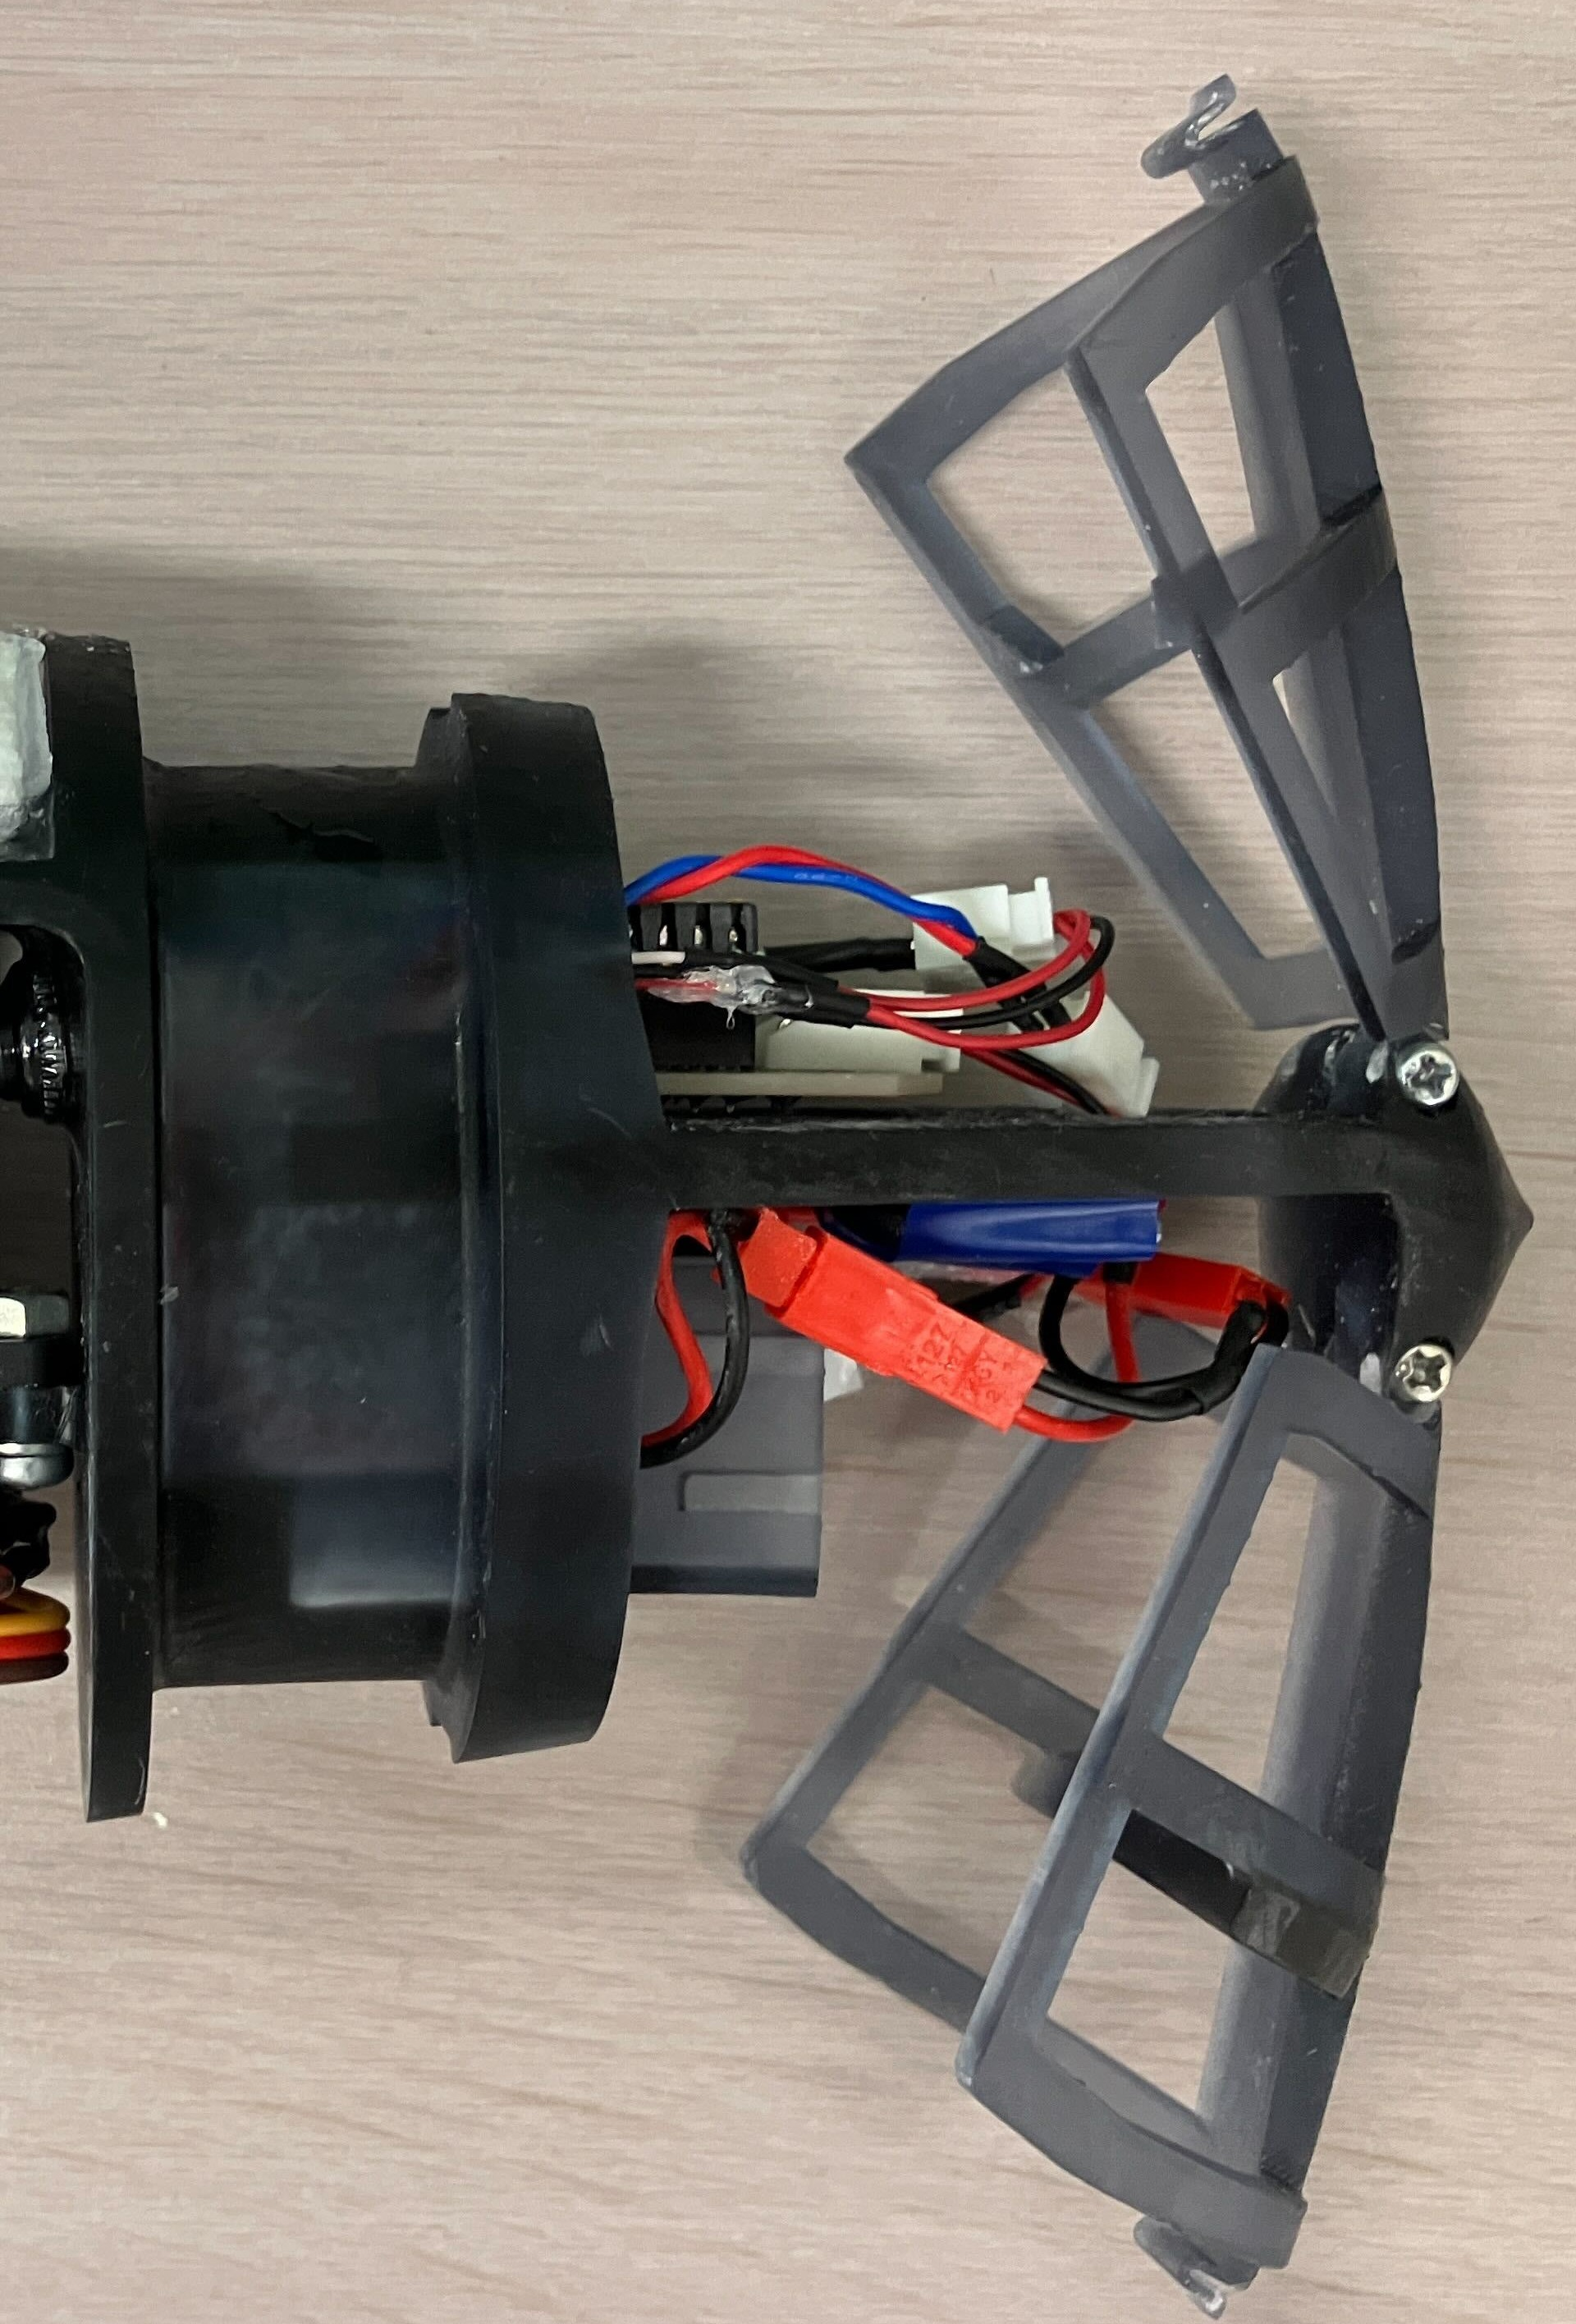
\includegraphics[width=0.4\linewidth]{chapters/picture/open_head.jpg}
        \caption{頭部開放時の様子}
        \label{fig:head_open}
    \end{minipage}
    \begin{minipage}[b]{0.44\linewidth}
        \centering
        \setPicture{rock.png}
        \caption{ワンタッチロックの仕組み}
        \label{fig:rock}
    \end{minipage}
\end{figure}
\begin{figure}[t]
    \centering
    \begin{minipage}[b]{0.35\linewidth}
        \centering
        \setPicture{toubu_kiban.png}
        \caption{基板固定方法}
        \label{fig:toubu_kiban}
    \end{minipage}
    \hspace{0.05\linewidth}
    \begin{minipage}[b]{0.35\linewidth}
        \centering
        \setPicture{toubu_battery.png}
        \caption{バッテリー固定方法}
        \label{fig:toubu_battery}
    \end{minipage}
\end{figure}

\subsection{胴体部}
胴体部は細かく分けて駆動部,弾性体部,尾びれ部で構成されている.
駆動部は頭部と一体化しており,試作機と同じサーボモータを配置し,プーリー(PLA樹脂)を取り付けている.昨年度卒業研究では頭部にサーボモータを配置していたが,今回は先行研究\cite{juu}で示さ
れた胴体後半部のみ体をしならせ遊泳するアジ型遊泳の特徴に従い,胴体後半部のみを屈曲できるような位置にサーボモータを配置した.
また,サーボモータの信号線を制御回路側につなげるために防水キャプコン(オーム電機,OA-WS04M-20/25)を配置し,さらに電源スイッチも配置している(図\ref{fig:kudou}).また,駆動部には
図\ref{fig:cover}のようなカバーをかぶせ魚らしい形状になるようにしている.

弾性体部は弾性体(ポリプロピレン板,厚さ0.75 mm)と骨格リンク(PLA樹脂),ワイヤ(ポリエステル製,0.40 mm)で構成している.骨格リンクは厚みを6mmで作製し,14 mm間隔を空
けながら配置した.リンクには図のようにワイヤを通すために2 mmの穴を4 カ所開けており,さらに胴体内部を浸水させるために大きめの穴を6 個開けている(図\ref{fig:link2}).また,リンクと弾性体は
ネジを用いて二点止めし,外皮の動きによってリンクがずれないように工夫した(図\ref{fig:real_link}).

尾びれ部は図\ref{fig:obire}のように尾びれ本体(ポリスチレン製薄板,厚さ0.3 mm)と骨格リンクの一部で構成している.尾びれに関しては先行研究\cite{ni}より推進性能が高いと示された材料と厚みを使用して
おり,形状に関してはアジの3Dスキャンデータからサイズを決定した.
\begin{figure}[hb]
    \centering
    \begin{minipage}[b]{0.32\linewidth}
        \centering
        \setPicture{kudou.png}
        \caption{駆動部のようす}
        \label{fig:kudou}
    \end{minipage}
    \hspace{0.1\linewidth}
    \begin{minipage}[b]{0.3\linewidth}
        \centering
        \setPicture{cover.jpg}
        \caption{駆動部カバー}
        \label{fig:cover}
    \end{minipage}
\end{figure}
\begin{figure}[hb]
    \centering
    \begin{minipage}[b]{0.30\linewidth}
        \centering
        \setPicture{link2.png}
        \caption{骨格リンクについて}
        \label{fig:link2}
    \end{minipage}
    \hspace{0.1\linewidth}
    \begin{minipage}[b]{0.33\linewidth}
        \centering
        \setPicture{link_danseita.jpg}
        \caption{実際の弾性体部}
        \label{fig:real_link}
    \end{minipage}
\end{figure}
\begin{figure}[t]
    \centering
    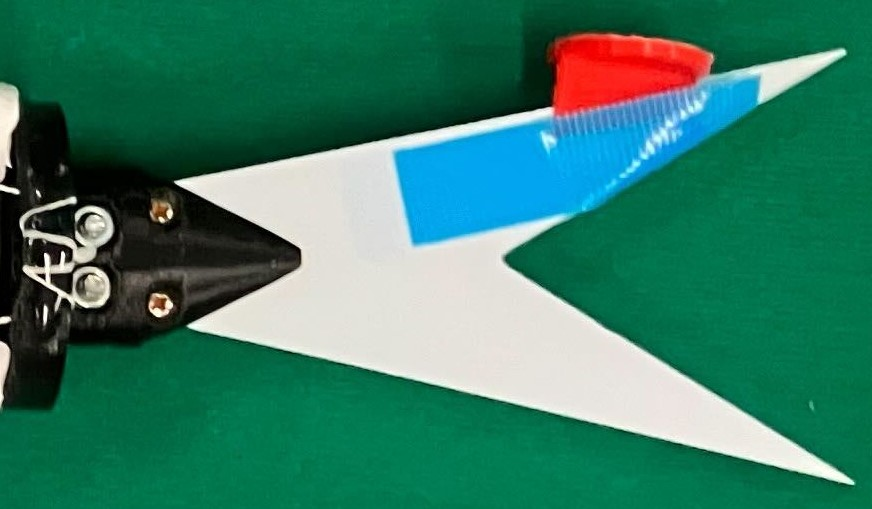
\includegraphics[width=0.5\linewidth]{chapters/picture/obire.jpg}
    \caption{尾びれ部}
    \label{fig:obire}
\end{figure}
骨格リンクは尾びれを固定するための固定部を設け,尾びれが折れないようにTPU樹脂で作製し,根元を三角形状にすることで折り目がつ
かないようにした.また,尾びれにはトラッキング用のマーカー(PLA樹脂)を取り付けた.

\subsection{柔軟外皮}
柔軟外皮は頭部と胴体部用に二つ作製した.今回は先行研究\cite{kyu}を参考に柔軟外皮を作製するため鋳造のように型にシリコン(Smooth-On社,ECOFLEX30)を流し入れることによって柔軟外皮の作成を行った.図\ref{fig:katanaka}に作製・使用した型
と中子をそれぞれ示す.ここで中子とは鋳造において中空部を作るために使われているもので, 型の間にはめ込んで使用する.この制作方法において柔軟外皮の外寸サイズを決定するのは型に作る
くぼみ,内寸サイズを決定するのは中子となる.したがってここから型のくぼみのサイズを柔軟外皮の外寸,中子のサイズを柔軟外皮の内寸と呼ぶ.

まず頭部用の柔軟外皮について,柔軟外皮の内寸は柔軟外皮と頭部が密着するようにアジの3Dモデルの頭部のサイズをそのまま使用した.外寸については体高方向に2 mm,体幅方向に3 mmの厚みになるよう
にアジのモデルデータの頭部をx軸方向に1.15 倍,y軸方向に1.09 倍,z軸方向に1.07 倍したサイズを使用した.

次に胴体部の柔軟外皮ついて述べる.リンクの動きに柔軟外皮を追従させるために柔軟外皮内部に骨格リンクをはめ込めるような溝を作製し,しわができないように柔軟外皮の内寸をロボットの胴体サイズの90 %
のサイズで作製した.サイズを小さめに作製することにより常に外皮にテンションがかかり,しわが寄らないようになった.溝の間隔もロボット胴体サイズの90 %になるようにリンク間距離14 mm
の90 %の長さにあたる12.6 mm間隔で作製した.溝の深さは骨格リンクに通すワイヤに干渉しないかつ溝から外れないように5 mmで設計した.
図\ref{fig:gaihi}に作製した柔軟外皮を示す.

胴体部の柔軟外皮はリンクを溝にはめ込むことである程度固定される.また柔軟外皮の頭部側の端を防水リングを締め付ける溝の部分にひっかける事によってさらに固定をしている(図\ref{fig:gaihi_kotei}の
赤丸の部分がひっかけている箇所).
\begin{figure}[t]
    \centering
    \begin{tabular}{cc}
        \begin{minipage}[b]{0.4\linewidth}
            \centering
            \setPicture{atata.jpg}
            \subcaption{頭部の柔軟外皮用の型と中子}
            \label{fig:atata} 
        \end{minipage}
        \hspace{0.05\linewidth}
        \begin{minipage}[b]{0.4\linewidth}
            \centering
            \setPicture{katata.jpg}
            \subcaption{胴体部の柔軟外皮用の型と中子}
            \label{fig:katata} 
        \end{minipage}
    \end{tabular}
    \caption{作製した型と中子}
    \label{fig:katanaka}
\end{figure}
\begin{figure}[ht]
    \centering
    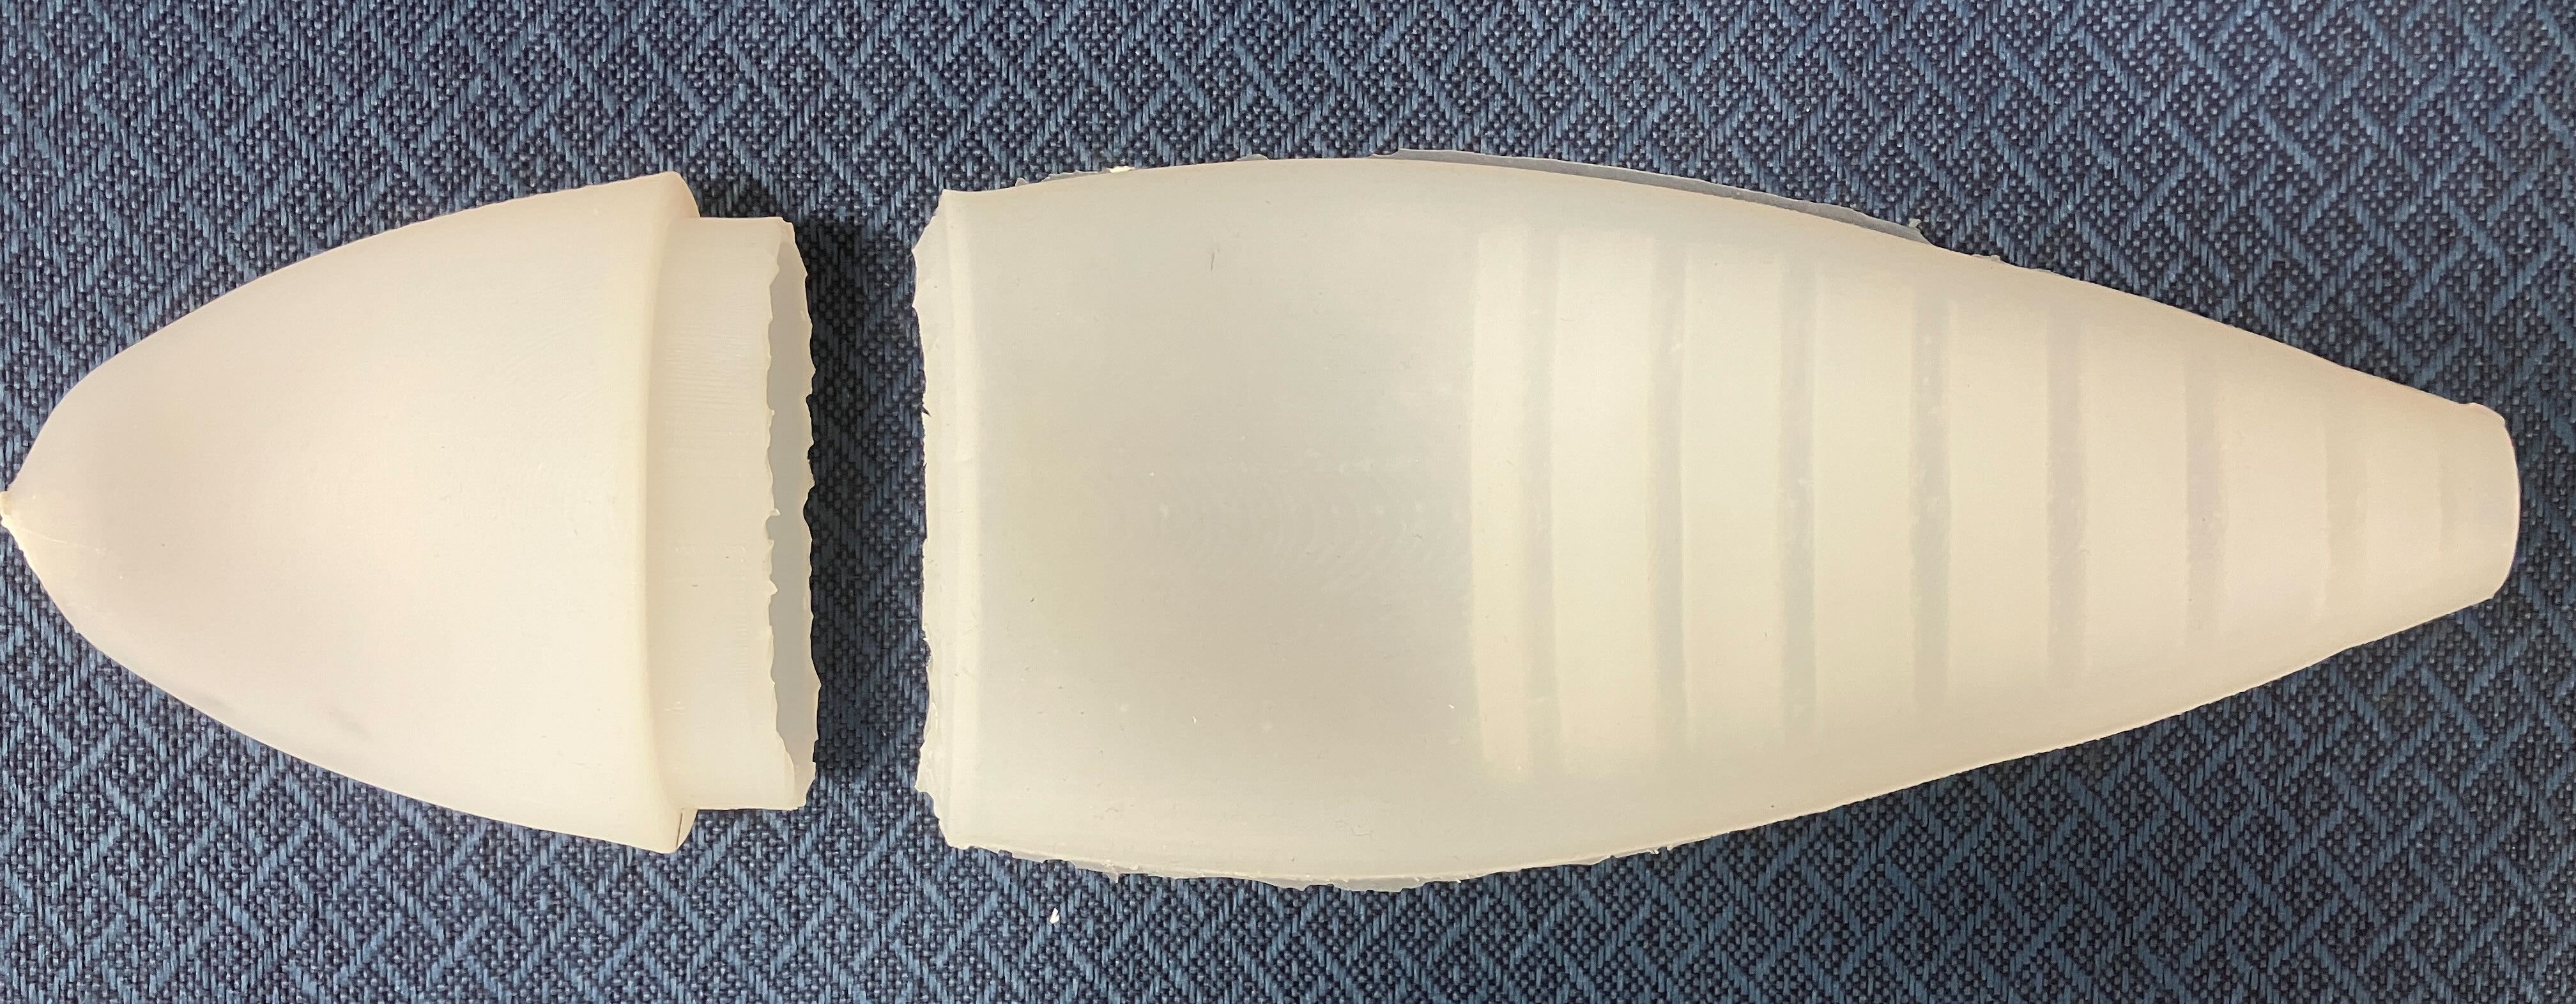
\includegraphics[width=0.8\linewidth]{chapters/picture/gaihi.jpg}
    \caption{作製した外皮}
    \label{fig:gaihi}
\end{figure}
\begin{figure}[t]
    \centering
    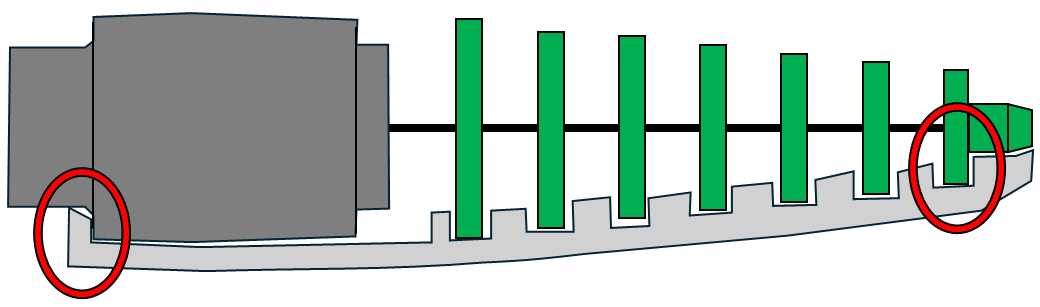
\includegraphics[width=0.7\linewidth]{chapters/picture/gaihi_kotei.png}
    \caption{胴体部の柔軟外皮の固定}
    \label{fig:gaihi_kotei}
\end{figure}